\chapter{Related Work} \label{cpt-related-work}

The proposed approach is an aggregation of a lot of ideas and implementations that have been 
around for quite some time. It is of great interest to explore related work which can provide 
context for use cases and highlight additional techniques that can adopted additionally. This 
chapter highlights related work adressing \emph{Voxel Rendering}, \emph{Occlusion Culling} 
and \emph{Mesh Shading}, which the proposed implementation is based on. The most important of 
the highlighted concepts are revisited and discussed in more detail in chapter 
\ref{cpt-technical-background}. 

[@TODO: Check redundancy with technological background]
[@TODO: Find scientific papers for voxel representations]

\section*{Voxel Representation} \label{sec-voxel-representation}

\begin{figure}[h]
    \centering
    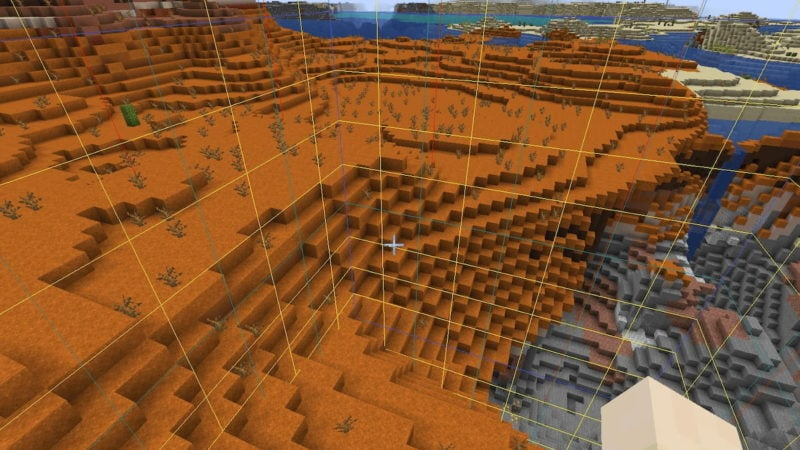
\includegraphics[width=300px]{images/graphics/minecraft-chunks.jpg}
    \caption{A screenshot from \emph{Minecraft}, with a debug visualization of the voxel chunks \cite{Palm2022}.}
    \label{fig:minecraft-chunks}
\end{figure}

\noindent
Voxel Rendering has had huge success in sandbox and highly dynamic games like \emph{Minecraft} (Mojang 
\cite{Mojang2024}, 2011) or \emph{Teardown} (Tuxedo Labs \cite{TuxedoLabs2022}, 2022). Usually these games try 
to preserve some volumetric information for the dynamic environment to be manipulated in real-time. \emph{Minecraft} 
generates a procedural environment based on complex parameters. This way, they can easily generate nearly infinie 
worlds with interesting biomes and landmarks. This huge world is split into chunks of size 16×384×16, to be able to 
stream the world dynamically and allow for quick traversal in any direction, shown in figure \ref{fig:minecraft-chunks}.
Each chunk maintains its own three-dimensional grid, with the voxel data being highly compressed. Non-existing voxels 
are not being stored, and block states, textures and other information is stored in per-chunk buffers or as global 
data in a global buffer. This way, using a texture atlas, up to 256 different texture variants can be easily stored 
per voxel by only one byte \cite{Bergensten2012, MinecraftFandom2021}. \\

\noindent
Many other games have made use of voxel rendering, adapting these principles of data compression and data streaming. 
Most optimizations rely on culling voxels which are not visible, e. g. faces that touch other faces.
Frustum culling and occlusion queries are also part of the optimization process, and partially used in \emph{Minecraft} 
as well, though the existance of frustum culling or the specific occlusion culling algorithm added in version 1.5 
cannot be confirm finally and reliably. Nevertheless, many efforts towards better performance have been made on the 
\ac{CPU} side. Lately, \ac{GPU}-driven approaches have been implemented by various individual developers. 
[@TODO: Find specific optimizations and sources!]  \\

\begin{figure}[h]
    \centering
    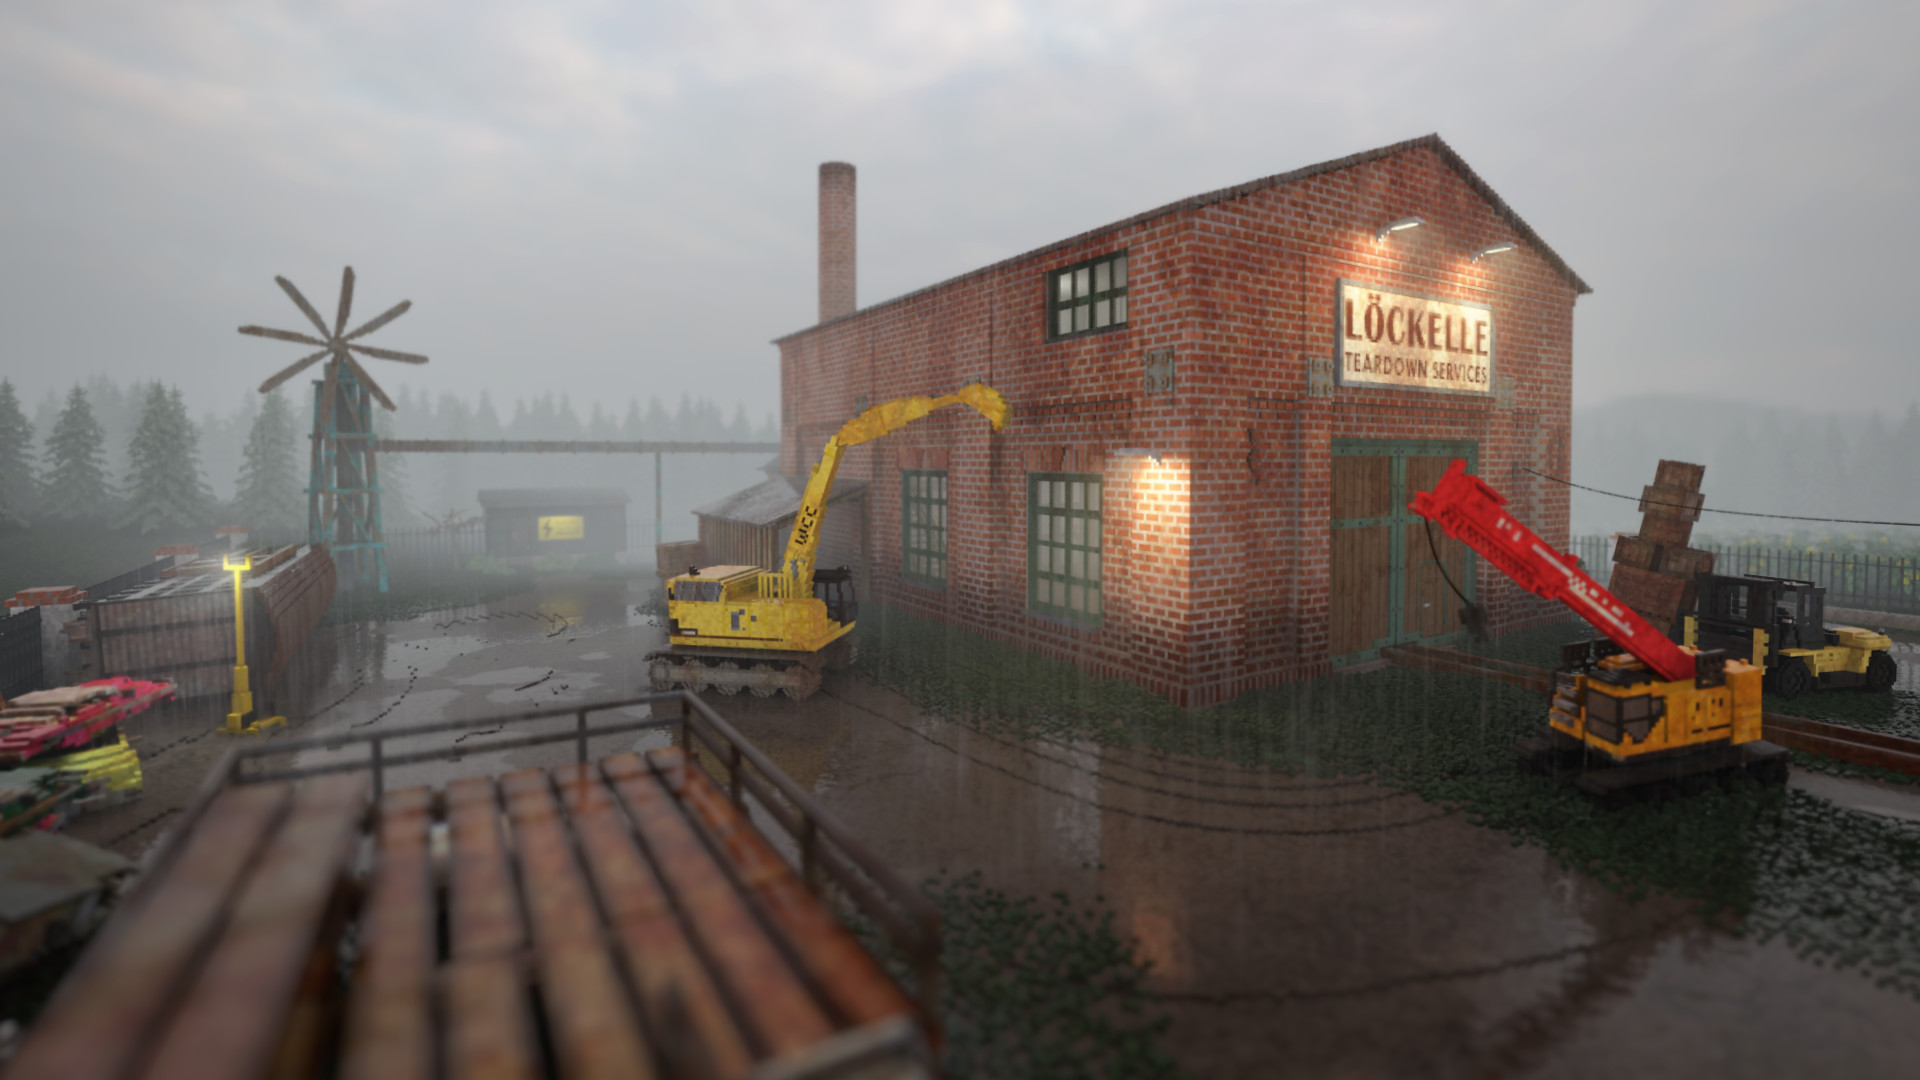
\includegraphics[width=300px]{images/graphics/teardown-ray-tracing.jpg}
    \caption{A screenshot from \emph{Teardown}, showcasing raytraced lighting \cite{TeardownSteam2022}.}
    \label{fig:teardown-raytracing}
\end{figure}

\subsection*{Sparse Voxel Directed Acyclic Graphs}

Kampe et al. \cite{Kampe2013} propose the use of their \emph{High-Resolution Sparse Voxel \ac{DAG}s}. This approach 
is tailored to high voxel resolutions and data that might not fit into memory all at once. Their data structure can 
be easily split up into several sub-trees, which in turn can be loaded individually. This approach seems promising 
for large scenes and use cases, which require the streaming of data. They propose to structure the data in a way that 
enables equal nodes of an octree hierarchy to be reduced to only one instance, eliminating redundant parts of the 
hierarchy and reducing the amount of used memory immensly. \\

\noindent
This approach relates to this implementation in how large voxelized scens can be efficiently loaded and stored in 
memory. Although this work doesn't explicitly rely on Sparse Voxel \ac{DAG}s, Sparse Voxel Octrees are used in the 
provoided implementation. Additionally, the proposed implementation can be optimized in the future to be working 
with Sparse Voxel \ac{DAG}s, enabling the handling of meshes with even higher resolution. \\

\noindent
Sparse Voxel \ac{DAG}s are not commonly used in rasterized rendering pipelines and store voxlumetric data in a binary 
format instead of storing positional data. This intoduces additional complexity to the pipeline which might result in 
better runtime performance but is also less intuitive when dealing with nodes and individual voxels. Sparse Voxel 
\ac{DAG}s mainly aim to provide a smaller memory footprint for raytraced applications while maintaining high resolution 
voxel meshes.


[@TODO: Add more related work for voxel representations]

\section*{Occlusion Culling}


\subsection*{Occlusion Queries}

The simplest method for testing visibility is the \ac{GPU} occlusion queries available in rendering \ac{API}s.
[@TODO: Find source and add what they found]

In the past, occlusion culling in games has been heavily influenced by \emph{Umbra} \cite{Umbra2024}, a company 
specialized on 3D occlusion culling solutions. \emph{Umbra} has been used by a lot of games such as 
\emph{Call of Duty: Ghosts} (2013), \emph{Killzone: Shadow Fall} (2013), \emph{Alan Wake} (2012) and many more 
\cite{UmbraWiki,CallOfDutyGhostsCredits,KillzoneUmbra,AlanWakeUmbra}. \emph{Umbra} voxelizes the game world and proceeds 
to process the data further, merging voxels into cells. A runtime hierarchy of the meshes inside the voxelgrid is created 
and subsequently, using the camera position, the cells can be queried for occlusion. As long as there are large 
occluders, this process can reduce the amount of instances and therefore the amount of triangles to draw. \emph{Umbra} 
also keeps a simplified depth buffer in memory in order to quickly determine visibility \cite{Medium2018}. The 
approach is similar to the approach provided in this work, in that both use a depth buffer and a scene hierarchy for 
computing visibility early in the pipeline. Both approaches rely on screen space bounding comparisons, although 
\emph{Umbra} uses a \emph{Portals and Cell} structure to manage visibility testing for a given camera position 
\cite{Medium2018}. Furthermore, \emph{Umbra} is usually applied in triangle mesh scene representations instead of 
volumetric, voxel-based scene representations. Another difference to this work's approach is the cell and portal 
structure, which needs to be traversed and kept in memory. \emph{Umbra} uses these structures for efficient 
visibility optimizations based on static scene meshes, while this work uses octree queries to dynamically determine 
possible occluders during runtime - or as a one time pre-computation for voxel models that are known to be static. \\



\subsection*{Two-Pass Occlusion Culling}

\noindent
\emph{Assassin's Creed Unity} (2014) uses a \ac{GPU} based two-pass occlusion culling technique as presented by 
Aaltonen et al. \cite{Aaltonen2015}. This technique involves both \ac{HZB} and depth reprojection. Both make for 
a good occlusion culling technique in games with large occluders or interiors. First, artist picked 
\emph{best occluders} are drawn to the depth buffer in a depth pre-pass. Then, projected bounding boxes can be 
used to test visibility of smaller objects in the scene. A hierarchical z-buffer is used to accelerate this testing,
as proposed by Greene et al. \cite{Greene93,Greene95}. Finally, the depth buffer of the last frame can be 
reprojected to further minimize computations. This technique allows developers to push for huge draw distances 
and densly crowded environments. Similar to this work, the game uses advanced technology in its implementation, 
clustering geometry and allowing for a \ac{GPU} centric approach of occlusion culling. However, the game doesn't 
use a volumetric representation but the standard boundary representation for its world. Furthermore, the best 
occluders are provided in different ways. Aaltonen et al. \cite{Aaltonen2015} propose the use of a hand-picked 
set of large, static meshes, while this work relies on a simple approximation of the voxel layout. This way, 
the latter implementation can dynamically provide best occluders in run-time, adapting the occlusion capabilities 
with the addition or removal of voxels in the scene.\\

\subsection*{Per-Meshlet Two-Pass Occlusion Culling}

Similar to \emph{Assassin's Creed Unity}, \emph{Alan Wake 2} (2023) and \emph{Unreal Engine 5} also implement \ac{HZB} 
and depth reprojection. Both implementations are directly based on the approach of Aaltonen et al. \cite{Aaltonen2015} 
but this time, making use of the new \emph{Mesh Shading} pipeline. The difference being the now provided hardware 
integration of clustering geometry \cite{Remedy2023,Karis2021}.  \\

\noindent
Karis et al. and Remedy Entertainment find, that using \ac{HZB} can provide great runtime performance for open, 
highly dense scenes. Both combine the \ac{HZB} with depth reprojection to further optimize the computation of the 
depth buffer. Using the Mesh Shading pipeline, this concept can be applied to meshlets, enabling per-meshlet culling. 
That means, that small parts of the geometry can be culled, even if other parts of the same mesh are still visible. 
This optimizes the culling further, so scenes can be more densly populated with meshes.\\

\noindent
The findings of Karis et al. and Remedy Entertainment are based on the works of Aaltonen et al. \cite{Aaltonen2015}
as well as Greene et al. \cite{Greene93,Greene95}. The same concept is adapted for this work's implementation and 
also relies on the use of the Mesh Shading pipeline.\\

\noindent
While the implementation of Karis et al. and Remedy Entertainment are based on a boundary representation and do not 
require the use of a spatial container for the culling algorithm, this implementation aims for another use case. 
In this work, voxels are used to represent the meshes and an additional spatial container is added to optimize the 
data further. 





\noindent [@TODO: Probably remove because its \ac{HZB}]
Another approach of applying occlusion culling is the \emph{raster occlusion culling}, proposed by \emph{NVIDIA}, among 
others \cite{NVIDIAGLOC2016}. The approach relies on "invisibly" rasterizing the objects as bounding boxes and using the 
rasterizer to query visibility checks and storing the per-object results in a visibility buffer. This buffer can then be 
used to draw the actual shaded objects and discard invisible objects. For the bounding boxes, only up to three faces are 
drawn in the early visibility check, to reduce load. Also, this can be optimized using instancing, the geometry shader or 
mesh shading to compute the visibility buffer efficiently \cite{NVIDIAGLOC2016}. This approach, especially when using 
mesh shading, is rather similar to the work employed here. However, the use case is different in a few details.


% SV DAGs
% AC Unity
% Alan Wake 2
% Greene
% Raster OC using depth queries -> not viable for so many objects